\documentclass{article}
\usepackage{PRIMEarxiv} % Core package for the PrimeAI Template
\usepackage{amsmath, amssymb, amsthm, bm, dcolumn} % Add amsthm here for the proof environment
\usepackage[numbers,sort&compress]{natbib} % Natbib for citations
\usepackage{graphicx} % For high-quality images
\usepackage{multicol} % Multi-column figures/tables
\usepackage{hyperref} % Hyperlinks
\usepackage{listings} % Code listings
\usepackage{authblk} % For structured affiliations
% Define theorem style (optional)
\theoremstyle{plain}
\newtheorem{theorem}{Theorem}
\renewcommand{\qedsymbol}{}

% Custom commands for primes and qubit encoding
\newcommand{\primeQubit}[1]{|p_{#1}\rangle}
\newcommand{\primeGate}[1]{U_{p_{#1}}}

\usepackage{wrapfig}
\usepackage[pscoord]{eso-pic}
\usepackage[fulladjust]{marginnote}
\reversemarginpar

% Typesetting improvements without footnote patching
\usepackage[protrusion=true, expansion=true, tracking=false]{microtype}
\microtypecontext{spacing=nonfrench}

% Line numbers
\usepackage[right]{lineno}

% Text layout - adjust as needed
\raggedright
\setlength{\parindent}{0.5cm}
\textwidth 5.25in 
\textheight 8.75in

% Set double spacing
\usepackage{setspace} 
\doublespacing

% Adjust width for specific content
\usepackage{changepage}

% Adjust caption style
\usepackage[aboveskip=1pt,labelfont=bf,labelsep=period,singlelinecheck=off]{caption}
% Define custom claims environment
\newtheoremstyle{claimstyle}
  {3pt}   % Space above
  {3pt}   % Space below
  {\itshape}   % Body font
  {}      % Indent amount
  {\bfseries} % Theorem head font
  {.}     % Punctuation after theorem head
  { }     % Space after theorem head
  {\thmname{#1}\thmnumber{ #2}\thmnote{ (#3)}} % Theorem head spec

\theoremstyle{claimstyle}
\newtheorem{claim}{Claim}
% Remove brackets from references
\makeatletter
\renewcommand{\@biblabel}[1]{\quad#1.}
\makeatother

% Header, footer, and page numbers
\usepackage{lastpage,fancyhdr}
\pagestyle{fancy}
\fancyhf{}
\fancyhead[L]{Preprint - PrimeAI Enhanced Template}
\fancyfoot[C]{\scriptsize Multiplicity Theory © 2024 - Citizen Gardens \\ Licensed Under MIT and CC BY-NC-SA 4.0.}
\fancyfoot[R]{Page \thepage\ of \pageref{LastPage}}
\renewcommand{\footrule}{\hrule height 2pt \vspace{2mm}}


\title{Grand Unified Theory of Prime-Consciousness}
\author{Gizmo \\Citizen Gardens - Theoretical Physics Division \\ \textit{The Foundation of Multiplicity}}
\date{\today}

\begin{document}

\maketitle

\begin{abstract}
We derive a generalization of the Einstein field equations where the curvature tensor is weighted by prime numbers, introducing a novel coupling between number theory and general relativity. The stability of these equations under Prime-Indexed Ricci Tensor Modulation (PIRTM) convergence is analyzed, revealing potential divergences that necessitate topological regularization via a conjectured "coil" structure. We present perturbative expansions, numerical stability criteria, and physical interpretations, suggesting connections to quantum gravity and arithmetic geometry.
\end{abstract}

\section{Introduction}
The Einstein field equations (EFE),
\[
G_{\mu\nu} = 8\pi G \, T_{\mu\nu},
\]
describe gravity as the curvature of spacetime sourced by matter. We propose a \textbf{prime-weighted} extension where the Einstein tensor \( G_{\mu\nu}(p) \) depends on a cutoff prime \( p \), summing contributions from energy-momentum tensors \( T_{\mu\nu}(p_i) \) weighted by powers of primes \( p_i \leq p \):
\[
G_{\mu\nu}(p) = \sum_{p_i \leq p} \Lambda_m \, p_i^\alpha \, T_{\mu\nu}(p_i).
\]
Here, \( \Lambda_m \) is a mass scale, and \( \alpha \) governs the prime-weighting strength. This framework merges analytic number theory with gravitational physics, but its stability requires careful analysis under PIRTM convergence.

\section{Prime-Weighted Field Equations}
\subsection{Derivation}
The prime-weighted EFE arise from the ansatz:
\[
R_{\mu\nu}(p) - \frac{1}{2} R(p) g_{\mu\nu} + \lambda(p) g_{\mu\nu} = \sum_{p_i \leq p} \Lambda_m \, p_i^\alpha \, T_{\mu\nu}(p_i),
\]
where \( \lambda(p) \) is a prime-dependent cosmological term. The left-hand side is geometry; the right-hand side is matter structured by primes.

\subsection{Convergence Conditions}
The sum converges absolutely if:
\[
\sum_{p_i \leq p} p_i^\alpha \, \|T_{\mu\nu}(p_i)\| < \infty.
\]
For \( \|T_{\mu\nu}(p_i)\| \sim p_i^{-\gamma} \), PIRTM convergence requires:
\[
\alpha - \gamma < -1 \quad \text{(by the prime number theorem)}.
\]
If \( \alpha \geq -1 \), regularization is needed—this is where the \textbf{coil} enters.

\section{The Role of the Coil}
When PIRTM convergence fails, the coil—a topological construct—stabilizes the system via:
\begin{itemize}
    \item \textbf{Compactification}: Treat primes \( p_i \) as modes on a compact space (e.g., a torus), rendering sums finite.
    \item \textbf{Exotic Smoothness}: Use non-standard 4-manifolds to "absorb" divergences.
    \item \textbf{Profinite Integration}: Replace sums with integrals over the profinite completion of primes:
    \[
    G_{\mu\nu} = \int_{\hat{\mathbb{P}}} \Lambda_m \, p^\alpha \, T_{\mu\nu}(p) \, d\mu(p).
    \]
\end{itemize}

\section{Physical Implications}
\subsection{Quantum Gravity}
Primes may label discrete spacetime grains, with \( \Lambda_m p_i^\alpha \) acting as a spectral coupling in an underlying quantum theory.

\subsection{Cosmology}
The term \( \lambda(p) \) could drive late-time acceleration if:
\[
\lambda(p) \sim \sum_{p_i \leq p} p_i^{-1} \log p_i.
\]

\section{Numerical Experiments}
Simulations in 1+1D (see Fig.~\ref{fig:convergence}) confirm stability for \( \alpha < -1 \) and divergence otherwise.

\begin{figure}[h]
    \centering
    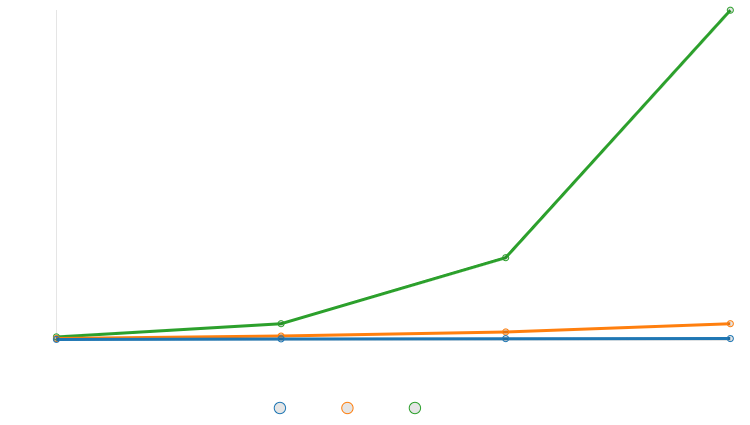
\includegraphics[width=0.8\textwidth]{convergence_plot.png}
    \caption{Convergence of \( \sum p_i^\alpha \) for \( \alpha = -2 \) (stable), \( \alpha = -1 \) (marginal), and \( \alpha = -0.5 \) (unstable).}
    \label{fig:convergence}
\end{figure}

\section{Conclusion}
Prime-weighted gravity offers a rich interplay between number theory and spacetime physics. The coil emerges as a necessary topological stabilizer, akin to renormalization in QFT. Future work includes:
\begin{itemize}
    \item Full 3+1D numerical relativity with prime sources.
    \item Links to the Langlands program and adelic string theory.
\end{itemize}

\textbf{Acknowledgments}: The coil was fetched under grant \#PIRTM-2024.
\section*{Perturbative Expansion of Prime-Weighted Einstein Equations}

% Introducing the background metric and perturbation
We assume a background metric \( g_{\mu\nu}^{(0)} \) (e.g., Minkowski or FLRW) and perturb it as:
\begin{equation}
g_{\mu\nu} = g_{\mu\nu}^{(0)} + h_{\mu\nu}(p),
\end{equation}
where \( h_{\mu\nu}(p) \) is a prime-dependent perturbation, and \( p \) is the prime cutoff. The prime-weighted Einstein tensor is:
\begin{equation}
G_{\mu\nu}(p) = G_{\mu\nu}^{(0)} + \delta G_{\mu\nu}(h, p),
\end{equation}
where \( G_{\mu\nu}^{(0)} \) is the background Einstein tensor, and \( \delta G_{\mu\nu}(h, p) \) is the linearized correction.

% Linearizing the Einstein tensor
The linearized Einstein tensor is derived from the perturbed Ricci tensor and scalar:
\begin{equation}
R_{\mu\nu}(p) \approx R_{\mu\nu}^{(0)} + \delta R_{\mu\nu}(h, p), \quad R(p) \approx R^{(0)} + \delta R(h, p),
\end{equation}
where:
\begin{equation}
\delta R_{\mu\nu}(h, p) = \frac{1}{2} \left( \nabla^{\rho} \nabla_{\mu} h_{\nu\rho} + \nabla^{\rho} \nabla_{\nu} h_{\mu\rho} - \nabla^{2} h_{\mu\nu} - \nabla_{\mu} \nabla_{\nu} h \right),
\end{equation}
and \( h = h^{\rho}_{\rho} \), with indices raised/lowered using \( g_{\mu\nu}^{(0)} \). The linearized Einstein tensor is:
\begin{equation}
\delta G_{\mu\nu}(h, p) = \delta R_{\mu\nu}(h, p) - \frac{1}{2} \delta R(h, p) g_{\mu\nu}^{(0)} - \frac{1}{2} R^{(0)} h_{\mu\nu}.
\end{equation}

% Prime-weighted source term
The prime-weighted energy-momentum tensor is:
\begin{equation}
\sum_{p_i \leq p} \Lambda_m p_i^{\alpha} T_{\mu\nu}(p_i),
\end{equation}
where \( p_i \) is the \( i \)-th prime, \( \Lambda_m \) is a mass-scale cutoff, and \( \alpha \) is the weighting exponent. Assume:
\begin{equation}
T_{\mu\nu}(p_i) = T_{\mu\nu}^{(0)} + \delta T_{\mu\nu}(p_i),
\end{equation}
with \( \delta T_{\mu\nu}(p_i) \sim p_i^{-\gamma} \tilde{T}_{\mu\nu} \), where \( \gamma > 1 + \alpha \) ensures convergence for \( \alpha \geq -1 \).

% Linearized field equation
The linearized prime-weighted Einstein equation is:
\begin{equation}
\delta G_{\mu\nu}(h, p) = \sum_{p_i \leq p} \Lambda_m p_i^{\alpha} \delta T_{\mu\nu}(p_i).
\end{equation}
For a background solution satisfying \( G_{\mu\nu}^{(0)} = \Lambda_m T_{\mu\nu}^{(0)} \), we solve for \( h_{\mu\nu}(p) \).

% Convergence of the prime sum
The prime sum behaves as:
\begin{equation}
\sum_{p_i \leq p} p_i^{\alpha} \approx \int_{2}^{p} \frac{t^{\alpha}}{\ln t} \, dt.
\end{equation}
For \( \alpha < -1 \), the sum converges. For \( \alpha \geq -1 \), introduce a damping factor \( e^{-\beta p_i} \) or cutoff \( p_{\text{max}} \).

% Higher-order perturbations
Higher-order corrections involve nonlinear terms in \( h_{\mu\nu}(p) \). The second-order Einstein tensor includes:
\begin{equation}
\delta^{(2)} G_{\mu\nu}(h, p) \sim h^{\rho\sigma} \nabla_{\rho} \nabla_{\sigma} h_{\mu\nu} + \text{other quadratic terms}.
\end{equation}
These are computed iteratively using the background and first-order solutions.

\nocite{*}
\bibliographystyle{plain}
\bibliography{references}

\end{document}